\documentclass{beamer}

\usepackage{beamerthemesplit}
\usetheme{Singapore} %Copenhagen}
%\usecolortheme{whale}

%\usepackage[T2A]{fontenc}
%\usepackage[utf8]{inputenc}
%\usepackage[russian]{babel}

\usepackage[main=russian,english]{babel}   %% загружает пакет многоязыковой вёрстки
\usepackage{fontspec}      %% подготавливает загрузку шрифтов Open Type, True Type и др.
\defaultfontfeatures{Ligatures={TeX},Renderer=Basic}  %% свойства шрифтов по умолчанию
\setmainfont{Times New Roman} %% задаёт основной шрифт документа
%\usefonttheme{professionalfonts}% SOLUTION
\usefonttheme{serif}

\usepackage{hyperref}
\usepackage{textcomp}
\usepackage{amssymb,amsmath}
%\usepackage{animate}
%\usepackage{longtable}
\usepackage{xcolor}

%\usepackage{pgffor}
\usepackage{enumitem}


\newcounter{N}

%% Форматирование окружения itemize
%\usepackage{ragged2e}
%\let\olditem\item
%\renewcommand\item{\olditem\justifying}


\newcommand{\argxi}{(\xi^1,\xi^2,\xi^3)}
\newcommand{\argx}{(x^1,x^2,x^3)}

\newcommand{\argxbarn}{(\bar{x}^1,\bar{x}^2,\ldots, \bar{x}^n)}
\newcommand{\argxn}{(x^1, x^2,\ldots, x^n)}

\newcommand{\argtxi}{(t, \xi^1,\xi^2,\xi^3)}
\newcommand{\argtoxi}{(t_0, \xi^1,\xi^2,\xi^3)}

\newcommand{\argtx}{(t, x^1,x^2,x^3)}
\newcommand{\argtox}{(t_0, x^1,x^2,x^3)}

\newcommand{\pd}[2]{\frac{\partial #1}{\partial #2}}
\newcommand{\pdk}[2]{\frac{\partial^2 #1}{\partial {#2}^2}}


\title[]{Законы сохранения механики сплошной среды}

\author[]{ {\em Верещагин Антон Сергеевич}
\\
канд. физ.-мат. наук, старший преподаватель\\
\bigskip
Кафедра аэрофизики и газовой динамики ФФ НГУ}

\usebackgroundtemplate{\includegraphics[width=\paperwidth]{../img/background.png}}

\begin{document}
	
\frame{\titlepage}


\frame{
	\frametitle{Аннотация}
	\parbox{\textwidth}{

	}
}

\frame{
	\frametitle{ Траектории движения точек и теорема об определителе }
	
		\begin{columns}
			\begin{column}{0.45\textwidth}
				\centering
				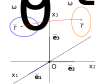
\includegraphics[width=\textwidth]{../img/omega_def.pdf}	
			\end{column}
			\begin{column}{0.55\textwidth}
%				\scriptsize
				\begin{exampleblock}{Иллюстрация перемещения сплошной среды}
					\parbox{\textwidth}{
					$\omega_0$, $\omega_t$ -- положение части сплошной среды в начальный момент времени и момент $t$.
					\[
					\vec{r}_0 = \xi^1\vec{e}_1+\xi^2\vec{e}_2+\xi^3\vec{e}_3,
					\]
					\[
					\vec{r} = x^1\vec{e}_1+x^2\vec{e}_2+x^3\vec{e}_3.
					\]
				}
				\end{exampleblock}				
			\end{column}
		\end{columns}
	

		\begin{exampleblock}{Траектории движения}
			\parbox{\textwidth}{
				Пусть траектории движения жидких частиц задаются функцией
				\[
					\vec{x} = \vec{x} \argtxi,
				\]
				где $\vec{\xi}$, $\vec{x}$ -- лагранжевы и эйлеровы координаты частицы.
			}
		\end{exampleblock}
	
	


	
}
\frame{
	\frametitle{ Определение траекторий по заданному полю движения }
		\begin{exampleblock}{Поле скоростей}
			\parbox{\textwidth}{
				Поле скоростей частиц сплошной среды в эйлеровой систем координат задаётся функцией $\vec{v}\argtx$. В лагранжевой системе координат скорость определяется соотношением
				\[
				\vec{v}\argtxi = \pd{\vec{x} \argtxi}{t}.
				\]
			}
		\end{exampleblock}

%					\vec{v} = \vec{v} \argtx

		\begin{exampleblock}{Задача определения траекторий движения по заданному полю скоростей}
		\parbox{\textwidth}{
			По заданному полю скоростей $\vec{v}\argtx$ требуется найти траектории движения частиц $x^i = x^i\argtxi$ с лагранжевыми координатами $\argxi$:
			\[
			\pd{x^i}{t} = v^i\argtx,\quad
			x^i |_{t=0} = \xi^i\quad
			(i=1,2,3).
			\]	
		}
	\end{exampleblock}
}

\frame{
	\frametitle{ Уравнения для нахождения матрицы Якоби }
	
	\begin{exampleblock}{Матричное уравнение на матрицу Якоби}
		\parbox{\textwidth}{
			Дифференцируя уравнения для нахождения траекторий по $\xi^j$ получим
			\[
			\pd{}{t} \pd{x^i}{\xi^j} = \pd{v^i}{x^k}\pd{x^k}{\xi^j},\quad
			\left. \pd{x^i}{\xi^j} \right|_{t=0}=\delta^i_j.
			\]
			
			Тогда матрица Якоби $y_{ij} = \displaystyle\pd{x^i}{\xi^j}$ удовлетворяет дифференциальному уравнению
			\[
			\pd{Y}{t}=AY,\quad Y|_{t=0} = E,
			\]
			где $A$ -- матрица, составленная из производных $\displaystyle\pd{v^i}{x^j}$, $E$ -- единичная матрица.
		}
	\end{exampleblock}
	
}

\frame{
	\frametitle{ Дифференцирование определителя матрицы Якоби }
	\parbox{\textwidth}{
	
		Обозначим $\Delta(t) = \operatorname{det Y(t)}$, тогда из определения определителя, как суммы произведений его элементов и правила дифференцирования произведения, имеем
		\[
		\Delta'(t) = \frac{d}{dt} 
		\left|
		\begin{array}{ccc}
		y_{11} & y_{12} & y_{13} \\
		y_{21} & y_{22} & y_{23} \\
		y_{31} & y_{32} & y_{33} \\
		\end{array}
		\right|=
		\]
		\[
		=		\left|
		\begin{array}{ccc}
		y'_{11} & y'_{12} & y'_{13} \\
		y_{21} & y_{22} & y_{23} \\
		y_{31} & y_{32} & y_{33} \\
		\end{array}
		\right|+
				\left|
		\begin{array}{ccc}
		y_{11} & y_{12} & y_{13} \\
		y'_{21} & y'_{22} & y'_{23} \\
		y_{31} & y_{32} & y_{33} \\
		\end{array}
		\right|+
				\left|
		\begin{array}{ccc}
		y_{11} & y_{12} & y_{13} \\
		y_{21} & y_{22} & y_{23} \\
		y'_{31} & y'_{32} & y'_{33} \\
		\end{array}
		\right|.
		\]
	}
	
}

\frame{
	\frametitle{ Дифференцирование определителя матрицы Якоби }

	\parbox{\textwidth}{
		Из матричного уравнения $\displaystyle\frac{dY}{dt}=AY$ следует, что
		\[
		y'_{1j} = a_{11}y_{1j}+a_{12}y_{2j} + a_{13}y_{3j},
		\]
		поэтому
		\[
		(y'_{11}, y'_{12}, y'_{13}) = a_{11}(y_{11}, y_{12}, y_{13})+
		a_{12}(y_{21}, y_{22}, y_{23})+
		a_{13}(y_{31}, y_{32}, y_{33}).
		\]
		Отсюда, вычитая из первой строки с производными линейную комбинацию остальных строк, имеем
		\[
		\left|
		\begin{array}{ccc}
			y'_{11} & y'_{12} & y'_{13} \\
			y_{21} & y_{22} & y_{23} \\
			y_{31} & y_{32} & y_{33} \\
		\end{array}
		\right|=
		\left|
		\begin{array}{ccc}
		a_{11} y_{11} & a_{11} y_{12} & a_{11} y_{13} \\
		y_{21} & y_{22} & y_{23} \\
		y_{31} & y_{32} & y_{33} \\
		\end{array}
		\right|=
		a_{11} \Delta(t).
		\]


	}


	
}

\frame{
	\frametitle{ Дифференцирование определителя матрицы Якоби }
	
	По аналогии можно получить, что
	\[
	\left|
	\begin{array}{ccc}
	y_{11} & y_{12} & y_{13} \\
	y'_{21} & y'_{22} & y'_{23} \\
	y_{31} & y_{32} & y_{33} \\
	\end{array}
	\right| = a_{22} \Delta(t),\quad
	\left|
	\begin{array}{ccc}
	y_{11} & y_{12} & y_{13} \\
	y_{21} & y_{22} & y_{23} \\
	y'_{31} & y'_{32} & y'_{33} \\
	\end{array}
	\right|=a_{33}\Delta(t).
	\]
	
	
	Таким образом,
	\[
	\Delta'(t) = (a_{11}+a_{22}+a_{33}) \Delta(t)=\operatorname{tr} A \, \Delta(t).
%	=	\pd{v^i}{x^i}\Delta(t) = \Delta(t) \operatorname{div} \vec{v} 
	\]
	
	\begin{exampleblock}{Правило дифференцирования определителя матрицы Якоби}
		\parbox{\textwidth}{
			\[
			\pd{}{t}\left| \pd{x^i}{\xi^j} \right| = \left| \pd{x^i}{\xi^j} \right|
			\left(
			\pd{v^1}{x^1}+\pd{v^2}{x^2}+\pd{v^3}{x^3}
			\right)=
			 \left| \pd{x^i}{\xi^j} \right|\operatorname{div} \vec{v}.
			\]
		}
	\end{exampleblock}
	
}

\frame{
	\frametitle{ Закон сохранения массы сплошной среды }
	\begin{columns}
		\begin{column}{0.45\textwidth}
			\centering
			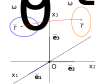
\includegraphics[width=\textwidth]{../img/omega_def.pdf}	
		\end{column}
		\begin{column}{0.55\textwidth}
		\begin{exampleblock}{Интегральный вид ЗСМ}
			\parbox{\textwidth}{
			\[
			\frac{d}{dt}\int\limits_{\omega_t}\rho\argtx d\vec{x} = 0,				
			\]
			где $\rho\argtx$ -- плотность жидкой частицы в точке $\vec{r}$ в момент времени $t$.
			}
		\end{exampleblock}		
		\end{column}
	\end{columns}
	
	
	\begin{exampleblock}{Упрощения}
		\parbox{\textwidth}{
		\[
		\frac{d}{dt}\int\limits_{\omega_t}\rho\argtx d\vec{x} = 
		\frac{d}{dt}\int\limits_{\omega_0}\rho\argtxi \Delta(t) d\vec{\xi}=
		\]
		\[
		=\int\limits_{\omega_0}\pd{}{t}\left(\rho\argtxi \Delta(t)\right) d\vec{\xi}=
		\]	
		}
	\end{exampleblock}
}

\frame{
	\frametitle{ Закон сохранения массы сплошной среды }
	\begin{exampleblock}{Упрощения}
		\parbox{\textwidth}{
		\[
		=
		\int\limits_{\omega_0}\left(\pd{\rho\argtxi}{t} \Delta(t) + \rho\argtxi\pd{\Delta(t)}{t} \right)d\vec{\xi}=
		\]
		\[
		=
		\int\limits_{\omega_0}\left(\pd{\rho\argtxi}{t}+ \rho\argtxi  \operatorname{div}_{\vec{x}} \vec{v} \right) \Delta(t) d\vec{\xi}=
		\]
		\[
		=\int\limits_{\omega_t}\left(\pd{\rho\argtx}{t}+ \rho\argtx  \operatorname{div}_{\vec{x}} \vec{v} \right) d\vec{x}.
		\]
		}
	\end{exampleblock}
	
	\begin{exampleblock}{ЗСМ в дифференциальной форме}
		\parbox{\textwidth}{
			В силу произвольности $\omega_t$
			\[
				\pd{\rho}{t}+ \rho \operatorname{div} \vec{v} = 0.			
			\]
		}
	\end{exampleblock}
	
}


\end{document}